\section{Вычислительные эксперименты}

    \subsection{Алгоритм}
        Для реализации моделей сделаем замену переменных \( u(t) = \dot{x}(t), \quad v(t) = \dot{y}(t) \), и получим систему дифференциальных уравнений первого порядка:
        \[
            \left\{\begin{split}
                & \dot{x} = u, & \dot{y} = v, \\
                & \dot{u} = 2 \Omega v, & \dot{v} = -2 \Omega u, \\
                & x(0) = x_0, & y(0) = y_0, \\
                & u(0) = x_1, & v(0) = y_1.
            \end{split}\right.
        \]

        Для компьютерного вычисления будем использовать метод Рунге-Кутты, с помощью которого получим численное решение системы дифференциальных уравнений с заданными параметрами. После чего построим их решения и фазовые плоскости.

        По полученному закону сохранения энергии можем вывести соотношение: \( u^2 + v^2 - x_1^2 - y_1^2 = 0 \). Также проверим его выполнение для численного решения. Для этого будем строить относительную погрешность на всём отрезке времени:
        \[
            \frac{u^2 + v^2 - x_1^2 - y_1^2}{x_1^2 + y_1^2}.
        \]



    \subsection{Программа}
        Для расчётов и визуализации был использован язык Python с библиотеками numpy и matplotlib.

        \lstinputlisting[language=Python,
        captionpos=t,
        style=colored,
        basicstyle=\footnotesize\dejavu,
        frame=lines]{src/4model.py}

    \subsection{Результаты}
        Построим траектории, выходящие из точки \( (5, 3) \) и имеющие начальные скорости: \( (0, 6), (5, 5), (1, 1), (-3, 3), (-4, -2), (1, -3) \) на отрезке времени \( [0, 5] \). Также покажем закон сохранения энергии.

        Для начала возьмём \( \Omega = 1 \).
        \begin{figure}[H]
            \centering
            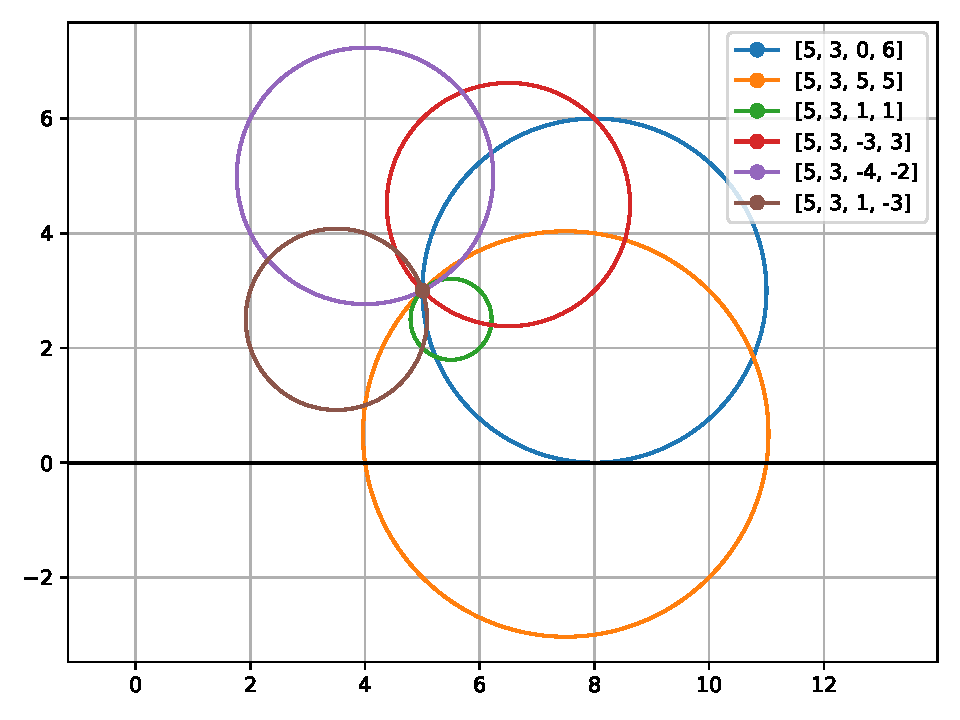
\includegraphics[width=8cm]{pictures/w1_3plot.pdf}
            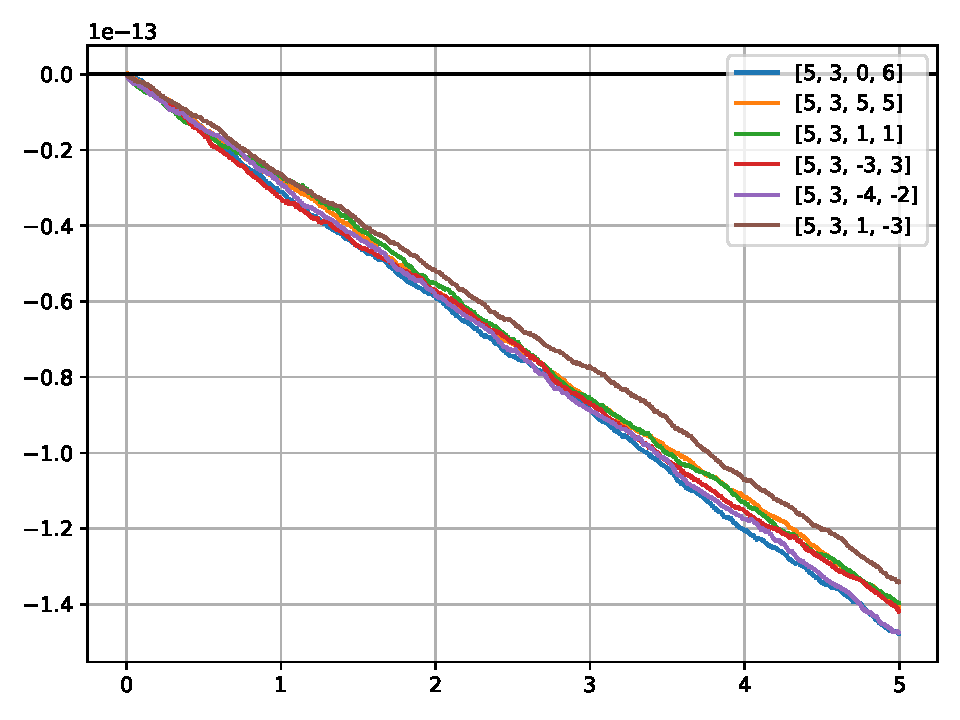
\includegraphics[width=8cm]{pictures/w1_3conv.pdf}
            \caption{Результат при количестве разбиений отрезка \( n = 2500 \).} \label{w1e3}
        \end{figure}

        \begin{figure}[H]
            \centering
            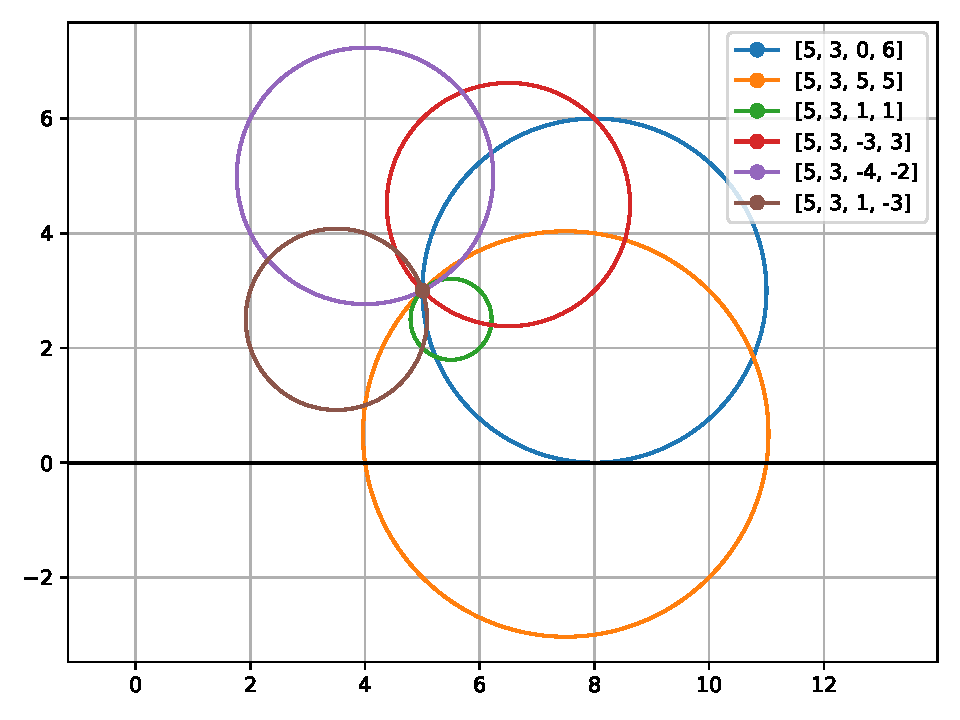
\includegraphics[width=8cm]{pictures/w1_3plot.pdf}
            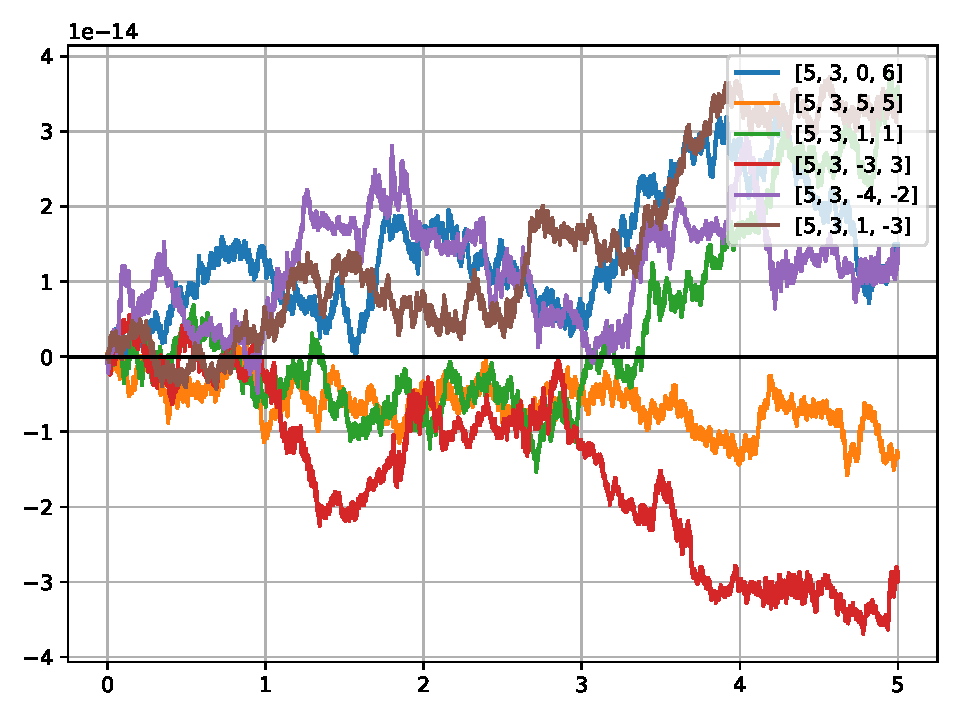
\includegraphics[width=8cm]{pictures/w1_5conv.pdf}
            \caption{Результат при количестве разбиений отрезка \( n = 100000 \).} \label{w1e5}
        \end{figure}

        Из графиков движения видно (Рис. \ref{w1e3}, \ref{w1e5}), что траекторией тела, которое находится во вращающейся системе координат, является окружность. Чем больше начальная энергия \( (u^2 + v^2) \), тем больше радиус окружности у траектории.

        У первого эксперимента с малым количеством разбиений отрезка времени погрешность увеличивается, из-за чего закон сохранения энергии не выполняется, хоть и сама погрешность по модулю небольшая. Это, вероятно, связанно с много большей погрешностью самого численного метода при меньшем количестве разбиений отрезка времени. У второго же, точностью больше и можно сказать, что соотношение выполняется с некоторой погрешностью.

        Теперь возьмём \( \Omega = 10 \).
        \begin{figure}[H]
            \centering
            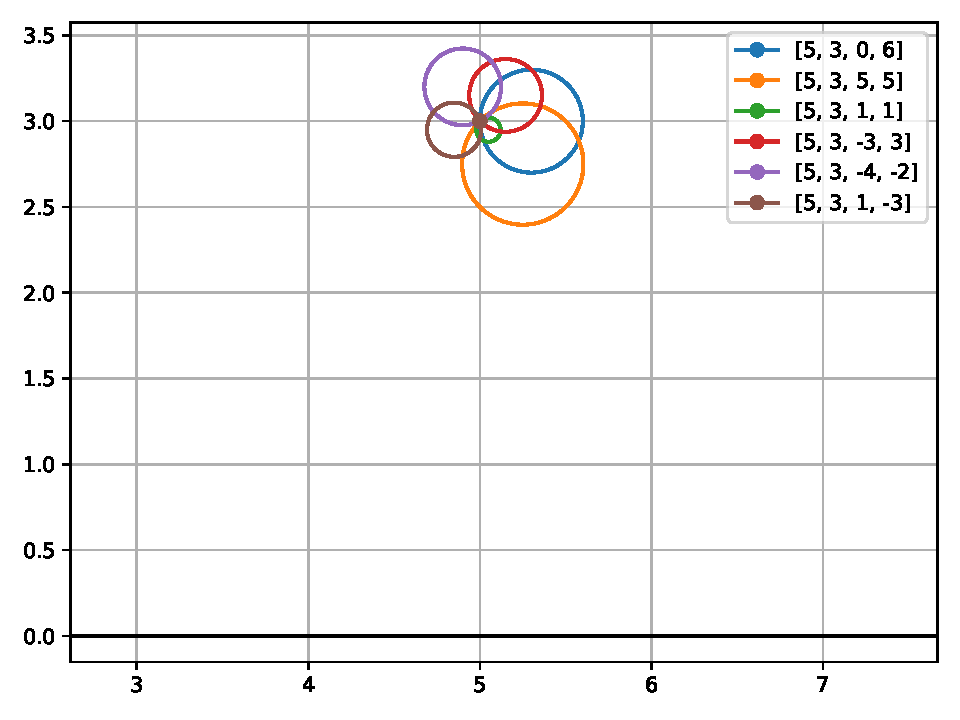
\includegraphics[width=10cm]{pictures/w10_3plot.pdf}
            \caption{Траектории при \( \Omega = 10 \).} \label{om10}
        \end{figure}

        \begin{figure}[H]
            \centering
            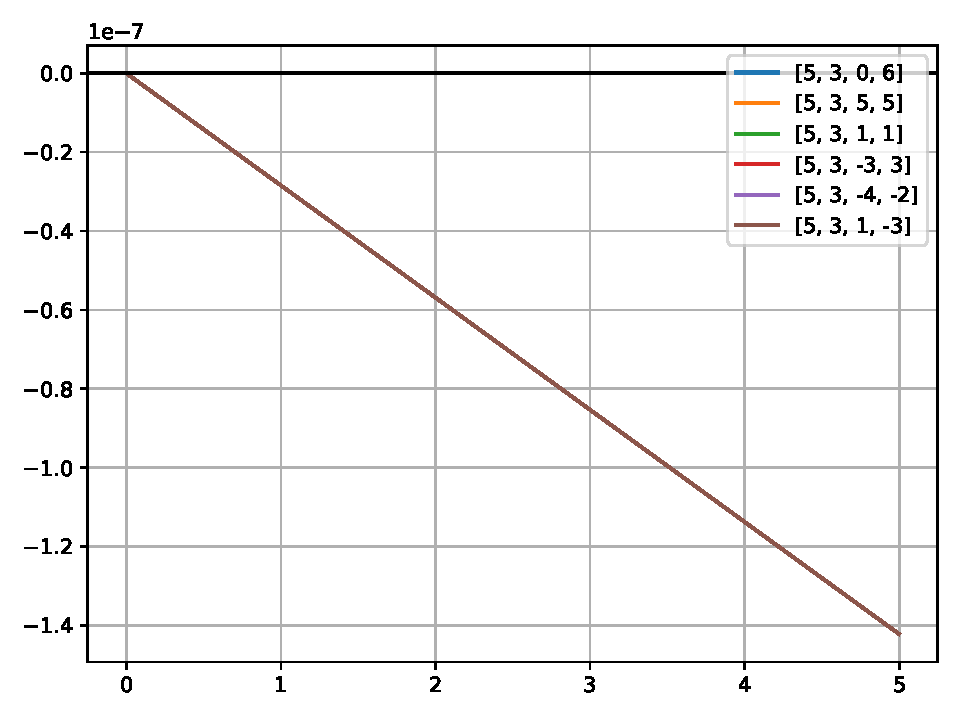
\includegraphics[width=8cm]{pictures/w10_3conv.pdf}
            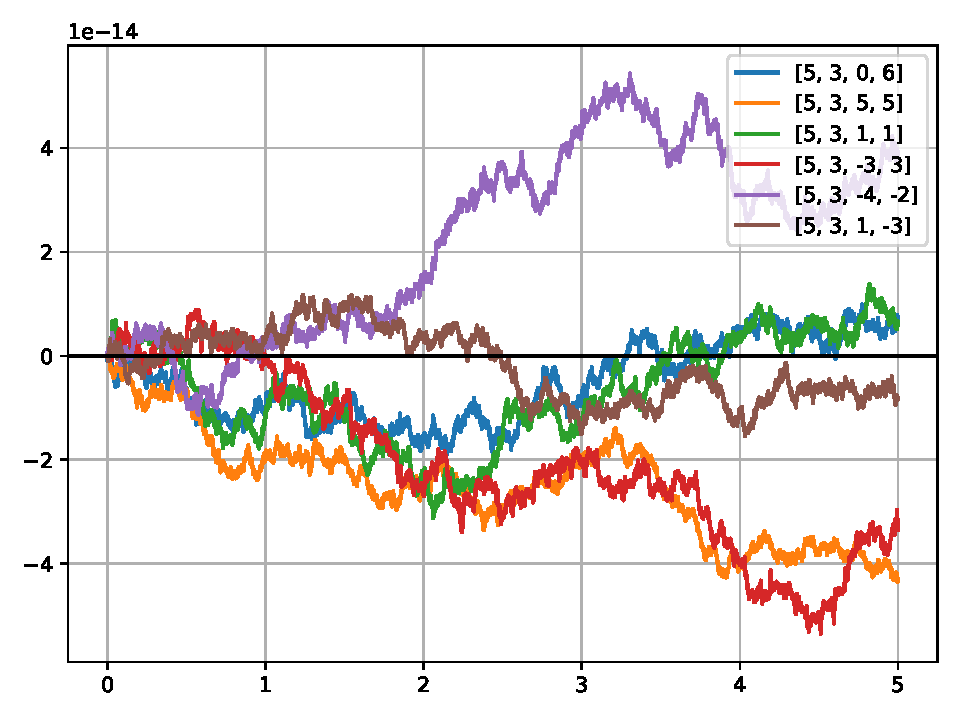
\includegraphics[width=8cm]{pictures/w10_5conv.pdf}
            \caption{Закон сохранения при количестве \( n = 2500 \) и \( n = 100000 \).}\label{om10conv}
        \end{figure}

        При большей угловой скорости вращения получаем окружности меньшего радиуса (Рис. \ref{om10}). Аналогично ведут себя результаты, показывающие закон сохранения энергии (Рис. \ref{om10conv}). При меньшем разбиении отрезка времени в данном эксперименте относительные погрешности становятся одинаковыми. При большем количестве разбиений закон аналогично выполняется с аналогичной погрешностью.
